\documentclass[conference]{IEEEtran}
\usepackage[utf8]{inputenc}
\usepackage[T1]{fontenc}
\usepackage[spanish,es-tabla]{babel}
\usepackage{cite}
\usepackage{amsmath,amssymb}
\usepackage{graphicx}
\usepackage{booktabs}
\usepackage{url}
\usepackage{microtype}

\renewcommand{\IEEEkeywordsname}{Palabras clave}

\begin{document}

\title{Caracterizaci{\'o}n visual y temporal de episodios de MP2,5 y clima en la Regi{\'o}n de Ays{\'e}n\\
\vspace{4pt}\large\textbf{EIN092B VISUALIZACI{\'O}N -- Profesor: Jorge Portilla}}

\author{
\IEEEauthorblockN{Maximiliano del R{\'i}o Linco{\~n}ir}
\IEEEauthorblockA{\textit{Departamento de Inform{\'a}tica}\\
\textit{Universidad T{\'e}cnica Federico Santa Mar{\'i}a}\\
Chile\\
mdelrio@usm.cl}
\and
\IEEEauthorblockN{Patricio Aylwin Retamal}
\IEEEauthorblockA{\textit{Departamento de Inform{\'a}tica}\\
\textit{Universidad T{\'e}cnica Federico Santa Mar{\'i}a}\\
Chile\\
paylwin@usm.cl}
}

\maketitle

\begin{abstract}
La contaminaci{\'o}n por material particulado fino (MP2,5) derivada de la combusti{\'o}n residencial de le{\~n}a constituye un problema cr{\'i}tico de salud p{\'u}blica en la Regi{\'o}n de Ays{\'e}n. Este trabajo dise{\~n}a y eval{\'u}a una arquitectura de an{\'a}lisis visual y de series de tiempo sobre 25 archivos horarios oficiales del SINCA (2013--2026) provenientes de cuatro estaciones: Coyhaique II, Coyhaique, Vialidad (Puerto Ays{\'e}n) y Cochrane. La metodolog{\'i}a incorpora una auditor{\'i}a expl{\'i}cita de datos faltantes y del a{\~n}o incompleto 2026 (corte 23 de octubre) mediante ventanas comparables acumuladas (ene--oct) e invernales (abr--sep), descomposici{\'o}n STL robusta, pruebas de tendencia de Mann--Kendall y pendiente de Sen, correlaci{\'o}n cruzada con variables meteorol{\'o}gicas, reducci{\'o}n de dimensionalidad mediante PCA y comparaci{\'o}n objetiva de algoritmos de agrupamiento y validaci{\'o}n explicativa temporal. En Coyhaique II, los d{\'i}as sobre la norma diaria de 50~$\mu$g/m$^3$ descendieron significativamente entre 2014 y 2025 ($p=0,002$; $-4,93$ d{\'i}as/a{\~n}o), aunque 2026 registr{\'o} un repunte invernal (99 d{\'i}as sobre norma), mientras Cochrane alcanz{\'o} 110 y 130 d{\'i}as en 2024--2025. Dentro del invierno, la velocidad del viento surge como el principal modulador meteorol{\'o}gico ($\rho=-0,686$). El modelo K-Means ($k=3$, estabilidad temporal ARI $=0,974$) aisl{\'o} un r{\'e}gimen fr{\'i}o-estancado que concentra el 76,5\% de todos los episodios. El aporte principal consiste en un flujo reproducible en Python, un prototipo interactivo y un modelo estrella listo para Power BI con criterios cuantitativos de selecci{\'o}n visual y anal{\'i}tica.
\end{abstract}

\begin{IEEEkeywords}
Calidad del aire, MP2,5, series de tiempo, visualizaci{\'o}n de datos, clustering.
\end{IEEEkeywords}

\section{Introducci{\'o}n}

En las ciudades del sur austral de Chile, las concentraciones de material particulado fino (MP2,5) superan de forma recurrente la norma primaria diaria de 50~$\mu$g/m$^3$ establecida por el Decreto Supremo N\textdegree~12/2011~\cite{mma2011ds12}, debido principalmente al uso intensivo de le{\~n}a para calefacci{\'o}n domiciliaria durante los meses fr{\'i}os~\cite{molina2017}. Coyhaique fue declarada zona saturada por MP2,5 en 2016~\cite{mma2016ds15} y mantiene promedios invernales que exceden los est{\'a}ndares nacionales e internacionales~\cite{solis2022}. Otras localidades de la Regi{\'o}n de Ays{\'e}n, como Puerto Ays{\'e}n y Cochrane, tambi{\'e}n cuentan con estaciones de monitoreo cuyas series son m{\'a}s cortas y presentan mayor proporci{\'o}n de vac{\'i}os o registros preliminares~\cite{sinca2026}.

El volumen y la naturaleza multivariada de estos registros ---m{\'a}s de 115.000 observaciones horarias por variable en Coyhaique II--- dificultan su inspecci{\'o}n directa en tablas est{\'a}ticas. Aunque el portal SINCA permite descargar cada serie por separado, no ofrece vistas integradas que comparen estaciones, separen componentes de tendencia y estacionalidad ni vinculen los episodios con la meteorolog{\'i}a local. Frente a esta brecha, el estudio aborda la siguiente pregunta de investigaci{\'o}n: \textit{{\textquestiondown}C{\'o}mo han evolucionado los episodios de MP2,5 en las ciudades de la Regi{\'o}n de Ays{\'e}n entre 2013 y 2026, y qu{\'e} condiciones meteorol{\'o}gicas se asocian a su ocurrencia?}

El objetivo general consiste en dise{\~n}ar y evaluar un conjunto de visualizaciones y modelos de series de tiempo que caractericen la evoluci{\'o}n y los reg{\'i}menes clim{\'a}ticos asociados al MP2,5 en Coyhaique, Puerto Ays{\'e}n y Cochrane. Los objetivos espec{\'i}ficos son: (1) describir patrones horarios, estacionales e interestacionales del MP2,5; (2) cuantificar la tendencia interanual y la frecuencia de d{\'i}as sobre norma controlando datos faltantes y el cierre parcial de 2026; y (3) relacionar los episodios con temperatura, viento, humedad y presi{\'o}n mediante correlaci{\'o}n cruzada, PCA y agrupamiento no supervisado.

Los resultados confirman una reducci{\'o}n hist{\'o}rica de episodios en Coyhaique y Puerto Ays{\'e}n, pero evidencian persistencia cr{\'i}tica en invierno ---con repunte en 2026--- y niveles severos en Cochrane. El resto del documento presenta los antecedentes (Secci{\'o}n~II), la metodolog{\'i}a (Secci{\'o}n~III), los resultados y discusi{\'o}n (Secci{\'o}n~IV) y las conclusiones (Secci{\'o}n~V).

\section{Antecedentes}

\subsection{Marco conceptual y antecedentes}
El MP2,5 corresponde a part{\'i}culas aerotransportadas de di{\'a}metro aerodin{\'a}mico inferior a 2,5~$\mu$m capaces de penetrar hasta los alv{\'e}olos pulmonares. En Chile, el DS N\textdegree~12/2011 fija un l{\'i}mite diario de 50~$\mu$g/m$^3$ (promedio de 24 horas con al menos 18 horas v{\'a}lidas) y define categor{\'i}as de Gesti{\'o}n de Episodios Cr{\'i}ticos (GEC): Regular (50--79), Alerta (80--109), Preemergencia (110--169) y Emergencia ($\geq$170~$\mu$g/m$^3$)~\cite{mma2011ds12}. Estudios previos en el centro-sur chileno muestran que las emisiones residenciales de biomasa dominan el inventario invernal~\cite{molina2017}, mientras que en Coyhaique el encajonamiento topogr{\'a}fico del valle favorece inversiones t{\'e}rmicas nocturnas que atrapan el humo cerca de la superficie~\cite{solis2022}.

\subsection{Estado del arte}
En la caracterizaci{\'o}n ambiental de ciudades patag{\'o}nicas y del centro-sur, Sol{\'i}s et al.~\cite{solis2022} evaluaron la serie 2014--2020 de Coyhaique mediante estad{\'i}sticos descriptivos est{\'a}ticos, documentando la concentraci{\'o}n invernal del MP2,5 sin abarcar otras localidades regionales ni a{\~n}os posteriores al Plan de Descontaminaci{\'o}n. Recientemente, Martinez-Soto et al.~\cite{martinez2025} analizaron la influencia meteorol{\'o}gica sobre el MP2,5 en Temuco, confirmando que las temperaturas bajas, la calma e{\'o}lica y la estabilidad atmosf{\'e}rica explican los episodios extremos en ciudades calefaccionadas con combustibles s{\'o}lidos.

Desde el an{\'a}lisis de series de tiempo, la descomposici{\'o}n STL (\textit{Seasonal-Trend decomposition using Loess})~\cite{cleveland1990stl} permite separar de manera robusta la tendencia de largo plazo, la estacionalidad anual y los residuos at{\'i}picos sin ser distorsionada por picos extremos~\cite{hyndman2021}. Para resumir variables correlacionadas y descubrir reg{\'i}menes sin{\'o}pticos se utilizan el An{\'a}lisis de Componentes Principales (PCA)~\cite{jolliffe2016} y m{\'e}todos de agrupamiento validados con {\'i}ndices internos como la silueta~\cite{rousseeuw1987}. En el plano visual, el marco de an{\'a}lisis de Munzner~\cite{munzner2014} y la jerarqu{\'i}a perceptual de Cleveland y McGill~\cite{cleveland1984} establecen que codificar magnitudes mediante posici{\'o}n sobre una escala com{\'u}n (series y barras) entrega mayor precisi{\'o}n que el color, reservando este {\'u}ltimo para grillas densas como los mapas de calor hora~$\times$~mes. El presente trabajo integra estas tres vertientes ---series de tiempo, agrupamiento multivariado y visualizaci{\'o}n interactiva orientada a Power BI--- sobre registros actualizados hasta octubre de 2026.

\section{Metodolog{\'i}a}

El c{\'o}digo reproducible, los guiones de auditor{\'i}a, el prototipo interactivo y el modelo estrella para Power BI se encuentran documentados en el repositorio del proyecto.\footnote{\url{https://github.com/MaksiiDR/aysen-mp25-visualizacion}}

\subsection{Datos, calidad, manejo de faltantes y a{\~n}o incompleto 2026}
Se reunieron 25 archivos CSV descargados del SINCA~\cite{sinca2026} en octubre de 2026: 22 series horarias de contaminantes y meteorolog{\'i}a y 3 tablas de frecuencias direccionales de viento, cubriendo Coyhaique II (sep. 2013--oct. 2026; 115.200 filas por variable), Coyhaique (mar. 2013--oct. 2026 en MP2,5), Vialidad en Puerto Ays{\'e}n (oct. 2017--oct. 2026) y Cochrane (mar. 2021--oct. 2026).

Siguiendo la prioridad oficial del SINCA, cada registro horario consolid{\'o} valores validados, preliminares y no validados conservando una etiqueta de trazabilidad y aplicando filtros de rango f{\'i}sico. La auditor{\'i}a inicial revel{\'o} tres aspectos cr{\'i}ticos que guiaron el preprocesamiento:
\begin{enumerate}
\item \textit{Completitud desigual:} En Coyhaique II, MP2,5 (98,9\%), MP10 (98,5\%), CO (97,6\%), SO$_2$ (97,7\%), O$_3$ (96,6\%) y las cuatro variables meteorol{\'o}gicas (91,5--99,2\%) muestran alta disponibilidad; en contraste, NO$_2$ (30,0\%), NO (9,2\%) y NO$_x$ (10,0\%) se excluyeron del an{\'a}lisis multivariado por superar el 70\% de vac{\'i}os. En Vialidad la meteorolog{\'i}a alcanza 60,6\% y en Cochrane la serie de MP2,5 presenta 78,6\% de completitud con 100\% de datos no validados o preliminares entre 2021 y 2023.
\item \textit{Regla diaria y a{\~n}o incompleto 2026:} Los promedios de 24~h solo se calcularon con $\geq$18 horas v{\'a}lidas (75\%)~\cite{mma2011ds12}, sin imputar huecos largos en las m{\'e}tricas normativas. Dado que todas las series cierran el 23 de octubre de 2026 (80,8\% del a{\~n}o calendario en Coyhaique II, con 16,6\% de d{\'i}as preliminares/no validados), el a{\~n}o 2026 se marc{\'o} como incompleto. Para compararlo sin sesgo frente a a{\~n}os anteriores se definieron tres vistas: a{\~n}os calendario completos ($\geq$75\% de d{\'i}as v{\'a}lidos, excluyendo 2026), ventana acumulada comparable YTD (1~ene--23~oct) y temporada invernal completa (abr--sep, con 100\% de cobertura en 2026 en Coyhaique y Vialidad, y 94,5\% en Cochrane).
\item \textit{Verificaci{\'o}n de direcci{\'o}n del viento:} La inspecci{\'o}n directa de los archivos confirm{\'o} que el dataset no posee direcci{\'o}n horaria del viento, sino tablas est{\'a}ticas agregadas de 24 sectores de 15\textdegree{} (suma verificada entre 100,0\% y 100,1\%) para Coyhaique II, Coyhaique y Vialidad (ausente en Cochrane). En consecuencia, la rosa de vientos se acot{\'o} al r{\'e}gimen climatol{\'o}gico hist{\'o}rico, mientras la asociaci{\'o}n con episodios se evalu{\'o} con la velocidad horaria y diaria del viento.
\end{enumerate}

\subsection{Arquitectura anal{\'i}tica: Python a Power BI}
Dado que el proyecto busca identificar patrones espaciotemporales m{\'a}s que operar un pron{\'o}stico en tiempo real, el flujo separa el procesamiento anal{\'i}tico preliminar en Python (limpieza, STL, correlaciones, PCA/clustering y prototipo interactivo en Plotly Dash) de la visualizaci{\'o}n ejecutiva final en Power BI. Para ello, el pipeline exporta un esquema estrella normalizado (\texttt{dim\_estacion}, \texttt{dim\_fecha} con banderas YTD/invierno y seis tablas de hechos pre-agregadas) junto a medidas DAX de cumplimiento DS~12, completitud y calidad.

\subsection{Series de tiempo, agrupamiento y validaci{\'o}n explicativa}
El an{\'a}lisis temporal combina cuatro t{\'e}cnicas: (a) descomposici{\'o}n \textit{STL} robusta mensual ($\text{periodo}=12$, suavizador estacional $=13$, comparada frente a la variante no robusta mediante la desviaci{\'o}n mediana absoluta de residuos), restringida a meses con $\geq$75\% de d{\'i}as v{\'a}lidos e interpolando {\'u}nicamente huecos aislados para la estimaci{\'o}n STL; (b) prueba no param{\'e}trica de \textit{Mann--Kendall} y pendiente de \textit{Sen} sobre promedios y conteos de d{\'i}as $>50$~$\mu$g/m$^3$; (c) funciones de autocorrelaci{\'o}n (ACF/PACF, rezagos 1--14 d{\'i}as) para medir persistencia de episodios; y (d) funci{\'o}n de correlaci{\'o}n cruzada de Spearman (CCF, rezagos $k\in[-5,+5]$ d{\'i}as) y pruebas de Mann--Whitney entre d{\'i}as episodio y normales.

Para agrupar d{\'i}as con perfiles afines en Coyhaique II ($n=3.949$ d{\'i}as completos, ago. 2015--oct. 2026), se estandarizaron seis variables con transformaci{\'o}n $\log(1+x)$ en contaminantes asim{\'e}tricos ($\log\text{MP2,5}$, $\log\text{CO}$, temperatura, humedad, velocidad del viento y presi{\'o}n) y se aplic{\'o} PCA~\cite{jolliffe2016}. Se compararon \textit{K-Means}, \textit{Gaussian Mixture Model} (GMM, covarianza completa) y agrupamiento jer{\'a}rquico de \textit{Ward} para $k\in\{2,\dots,6\}$ usando tres m{\'e}tricas internas (Silueta~\cite{rousseeuw1987}, Davies--Bouldin y Calinski--Harabasz) m{\'a}s estabilidad temporal (Adjusted Rand Index, ARI, entrenando en la primera mitad 2015--2020 y evaluando en 2021--2026).

De modo complementario, para cuantificar objetivamente cu{\'a}nto explica la meteorolog{\'i}a (sola o junto a la persistencia $\text{MP2,5}_{t-1}$) la ocurrencia de d{\'i}as $>50$~$\mu$g/m$^3$, se contrastaron tres clasificadores ---Regresi{\'o}n Log{\'i}stica, Random Forest y Gradient Boosting--- frente a una l{\'i}nea base de persistencia ($t-1$). Los hiperpar{\'a}metros se ajustaron mediante \texttt{GridSearchCV} con validaci{\'o}n cruzada temporal \texttt{TimeSeriesSplit} (5 particiones, optimizando F1) sobre 2015--2023 ($n=2.982$) y se evaluaron fuera de muestra en 2024--2026 ($n=1.021$, 28,1\% d{\'i}as episodio) mediante F1, PR-AUC y ROC-AUC.

\subsection{Criterios objetivos de selecci{\'o}n visual}
Se evaluaron cuatro vistas candidatas (series temporales con tendencia STL, barras apiladas GEC, mapa de calor hora~$\times$~mes y calendario diario de 13 a{\~n}os) con una matriz de cuatro criterios (escala 1--3): precisi{\'o}n perceptual seg{\'u}n~\cite{cleveland1984}, claridad interpretativa, escalabilidad medida emp{\'i}ricamente sobre 115.200 registros horarios (umbral $<15$~s) y cobertura de objetivos espec{\'i}ficos.

\section{Resultados y Discusi{\'o}n}

\subsection{Resultados}
\begin{figure*}[t]
\centering
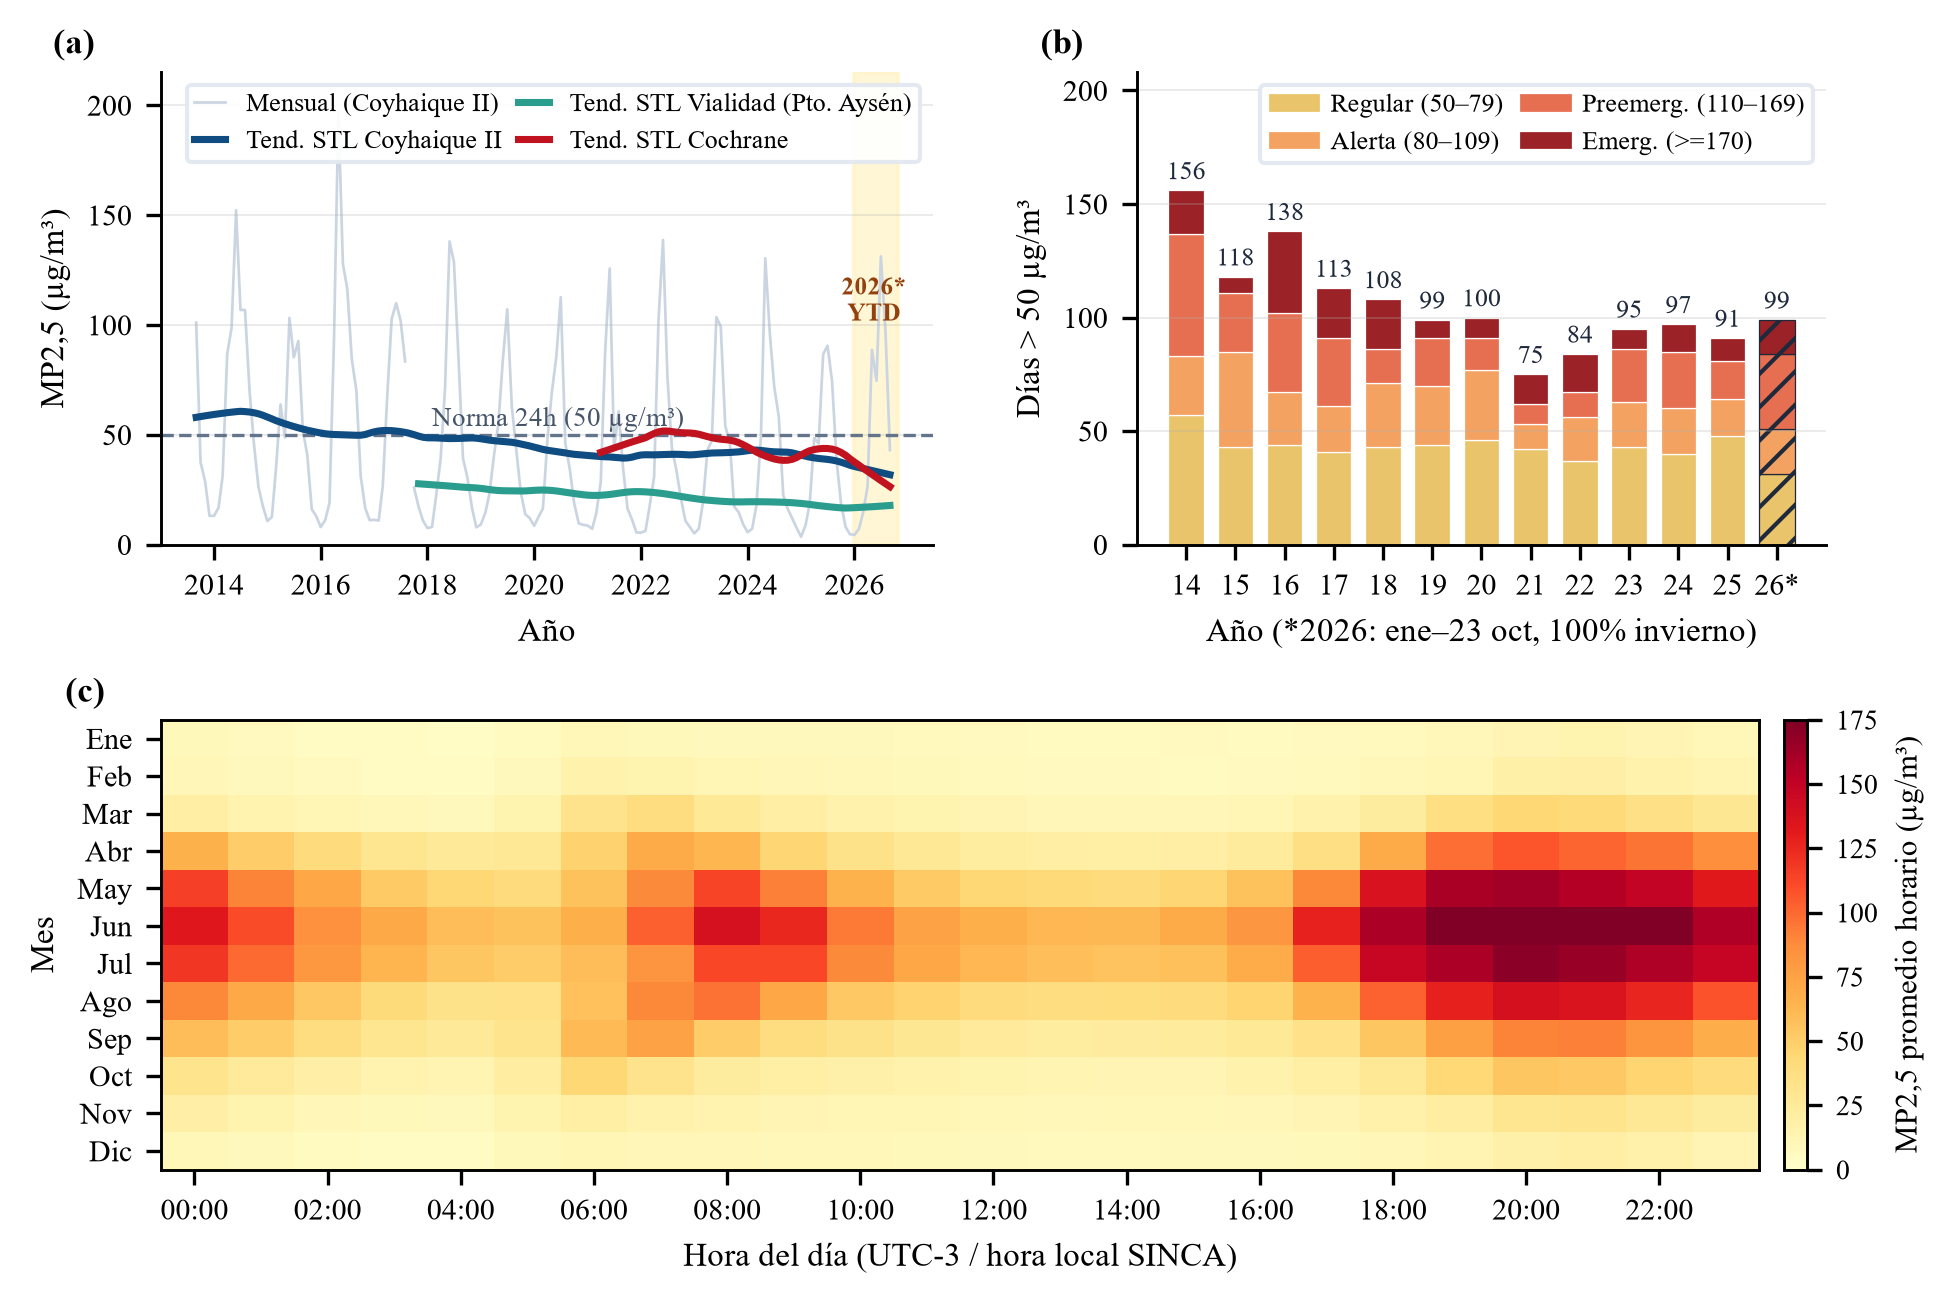
\includegraphics[width=\textwidth]{figures/fig1_temporal_patterns.png}
\caption{Evoluci{\'o}n temporal y patrones de MP2,5 en la Regi{\'o}n de Ays{\'e}n (2013--2026). (a) Promedio mensual de Coyhaique II y tendencia STL robusta para Coyhaique II, Vialidad (Puerto Ays{\'e}n) y Cochrane, indicando el l{\'i}mite diario DS~12 (50~$\mu$g/m$^3$) y el corte parcial de 2026 (ene--23 oct). (b) D{\'i}as sobre norma en Coyhaique II desglosados por categor{\'i}a GEC; la barra achurada de 2026* cubre el 100\% del invierno. (c) Mapa de calor del promedio horario de MP2,5 (hora~$\times$~mes) en Coyhaique II.}
\label{fig:temporal}
\end{figure*}

La Fig.~\ref{fig:temporal} resume la din{\'a}mica temporal del MP2,5. En los 4.761 d{\'i}as v{\'a}lidos de Coyhaique II se registraron 1.412 d{\'i}as sobre norma (29,7\% del total) y 202 emergencias ($\geq$170~$\mu$g/m$^3$), con un m{\'a}ximo diario de 945,0~$\mu$g/m$^3$. La estaci{\'o}n Coyhaique mostr{\'o} un comportamiento casi id{\'e}ntico (1.430 d{\'i}as $>50$~$\mu$g/m$^3$, 28,9\%; correlaci{\'o}n de Spearman $\rho=0,958$ con Coyhaique II en $n=4.732$ d{\'i}as). Vialidad present{\'o} niveles sustancialmente menores (300 d{\'i}as $>50$, 9,5\% en 3.162 d{\'i}as v{\'a}lidos; solo 1 emergencia), mientras Cochrane acumul{\'o} 564 d{\'i}as sobre norma en 1.609 d{\'i}as v{\'a}lidos (35,1\%, 31 emergencias), alcanzando 110 y 130 d{\'i}as $>50$ en los {\'u}nicos dos a{\~n}os completos y mayoritariamente validados (2024 y 2025). Pese a las diferencias de magnitud, las series diarias est{\'a}n fuertemente sincronizadas entre ciudades: Coyhaique II correlaciona con Vialidad ($\rho=0,829$, $n=3.148$) y con Cochrane ($\rho=0,822$, $n=1.606$, $p<0,001$).

En la descomposici{\'o}n STL (Fig.~\ref{fig:temporal}a), la fuerza estacional domin{\'o} en todas las estaciones (0,807 en Coyhaique II; 0,803 en Coyhaique; 0,945 en Vialidad y Cochrane). La opci{\'o}n robusta redujo casi a la mitad la desviaci{\'o}n mediana absoluta de los residuos en Coyhaique II (2,81 frente a 5,01~$\mu$g/m$^3$ en la versi{\'o}n no robusta). La tendencia STL descendi{\'o} de 57,95 a 31,82~$\mu$g/m$^3$ en Coyhaique II y de 27,69 a 17,82~$\mu$g/m$^3$ en Vialidad. La prueba de Mann--Kendall sobre a{\~n}os completos en Coyhaique II (2014--2025) confirm{\'o} una disminuci{\'o}n estad{\'i}sticamente significativa tanto en el promedio anual ($p=0,0075$; pendiente de Sen $-1,83$~$\mu$g/m$^3$/a{\~n}o) como en d{\'i}as $>50$ ($p=0,0020$; $-4,93$ d{\'i}as/a{\~n}o), pasando de 156 d{\'i}as en 2014 a un m{\'i}nimo de 75 en 2021 (Fig.~\ref{fig:temporal}b). Al incorporar 2026 mediante la ventana YTD (ene--23 oct, que contiene el 99,7\% de los episodios hist{\'o}ricos), la tendencia decreciente en d{\'i}as $>50$ se mantiene ($p=0,0049$; $-3,75$ d{\'i}as/a{\~n}o), pero el promedio invernal de 2026 repunt{\'o} a 77,5~$\mu$g/m$^3$ (99 d{\'i}as $>50$, con 33 preemergencias y 15 emergencias frente a 17 y 10 en 2025), dejando la tendencia de la media invernal en el l{\'i}mite de significancia ($p=0,0586$). En Vialidad, el invierno 2018--2026 descendi{\'o} significativamente ($p=0,0211$; $-4,38$ d{\'i}as/a{\~n}o, bajando de 61 a 16 d{\'i}as). Cochrane no mostr{\'o} tendencia significativa ($p>0,30$, solo 4 inviernos comparables).

El mapa de calor hora~$\times$~mes de Coyhaique II (Fig.~\ref{fig:temporal}c) exhibe una estacionalidad extrema: el promedio horario invernal (abr--sep) es de 77,7~$\mu$g/m$^3$ frente a 15,1~$\mu$g/m$^3$ entre octubre y marzo (raz{\'o}n $5,1\times$). En el ciclo diario invernal destacan dos m{\'a}ximos: uno matutino cercano a las 08:00~h y el principal en horario nocturno entre las 18:00 y 00:00~h, con un m{\'a}ximo promedio de 141,1~$\mu$g/m$^3$ a las 20:00~h (191,8~$\mu$g/m$^3$ en junio a las 21:00~h) frente a un m{\'i}nimo vespertino de 40,0~$\mu$g/m$^3$ a las 14:00~h.

\begin{figure*}[t]
\centering
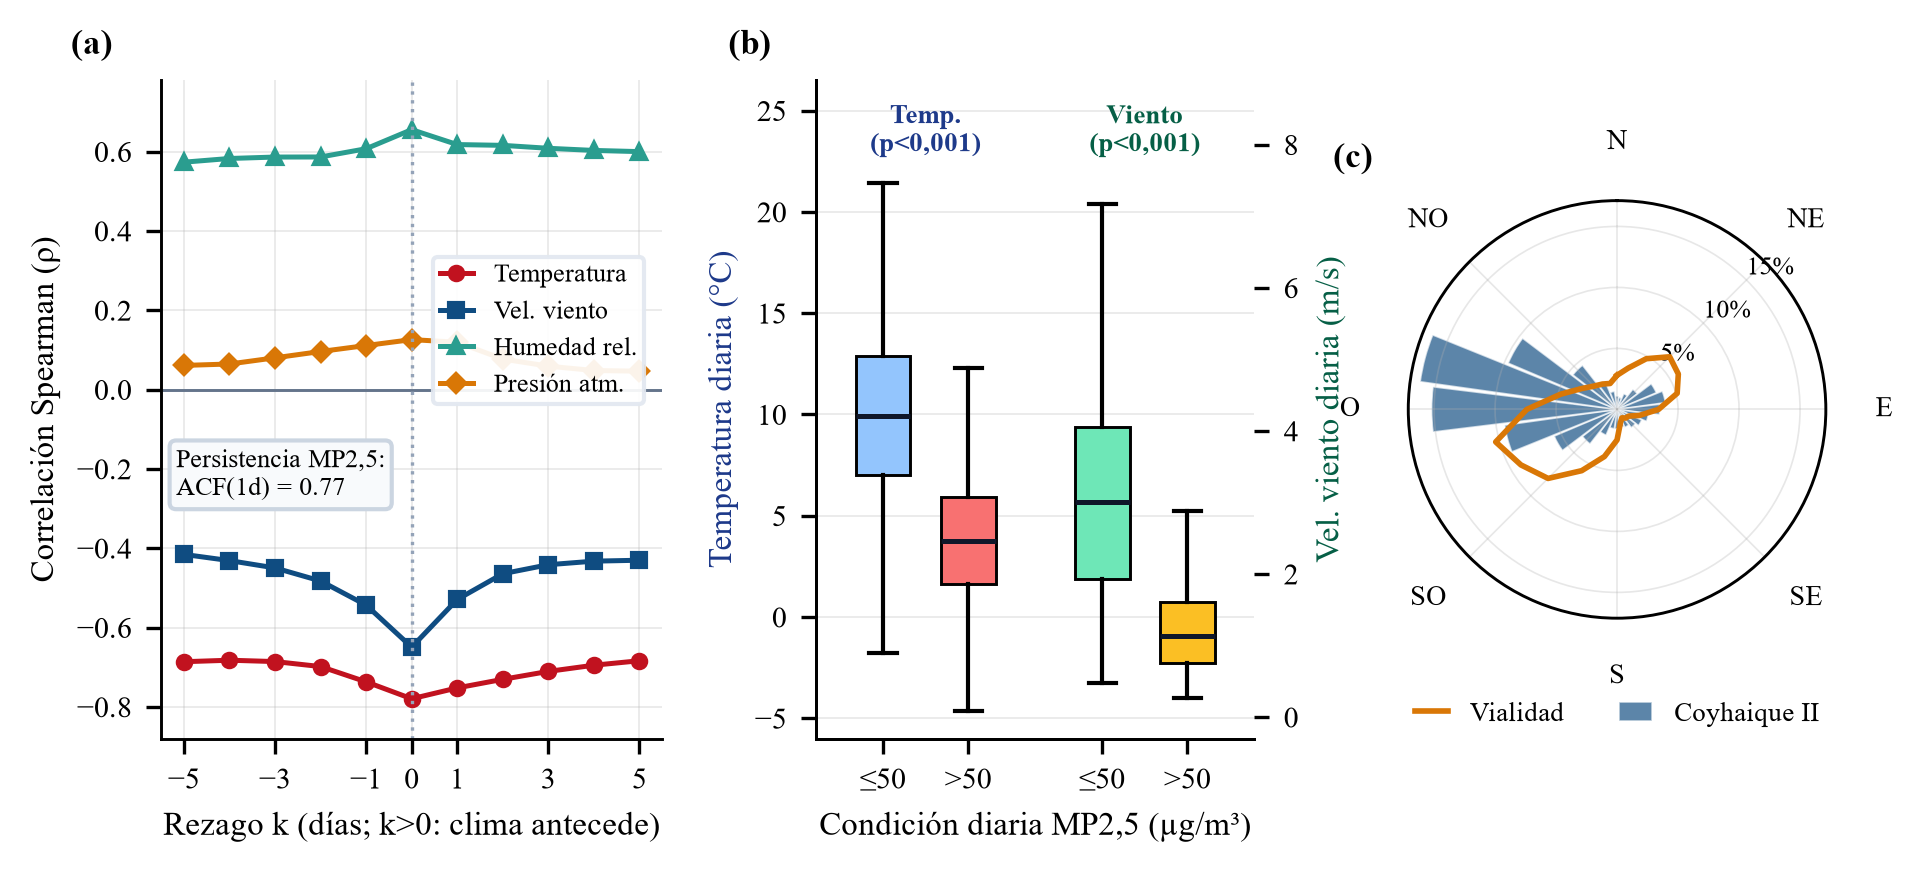
\includegraphics[width=\textwidth]{figures/fig2_meteorology_wind.png}
\caption{Relaci{\'o}n entre meteorolog{\'i}a, persistencia y MP2,5 en Coyhaique II (2013--2026). (a) Correlaci{\'o}n cruzada de Spearman (CCF) entre variables meteorol{\'o}gicas en $t-k$ y MP2,5 diario en $t$, junto a la autocorrelaci{\'o}n diaria de primer orden $\text{ACF}(1)=0,77$. (b) Distribuci{\'o}n diaria de temperatura y velocidad del viento en d{\'i}as normales ($\leq 50$~$\mu$g/m$^3$) frente a d{\'i}as episodio ($>50$~$\mu$g/m$^3$, Mann--Whitney $p<0,001$). (c) Rosa de vientos climatol{\'o}gica hist{\'o}rica por 24 sectores de 15\textdegree{} en Coyhaique II y Vialidad.}
\label{fig:met}
\end{figure*}

La Fig.~\ref{fig:met} detalla la asociaci{\'o}n meteorol{\'o}gica. En la serie diaria anual de Coyhaique II (Fig.~\ref{fig:met}a), las correlaciones contempor{\'a}neas ($k=0$) alcanzan $\rho=-0,780$ con temperatura, $\rho=-0,650$ con velocidad del viento, $\rho=+0,655$ con humedad relativa y $\rho=+0,126$ con presi{\'o}n atmosf{\'e}rica; al restringir el c{\'a}lculo exclusivamente a invierno (abr--sep), la velocidad del viento pasa a ser la variable m{\'a}s correlacionada ($\rho=-0,686$), superando a temperatura ($\rho=-0,512$), humedad ($\rho=+0,443$) y presi{\'o}n ($\rho=+0,183$). La autocorrelaci{\'o}n diaria del MP2,5 es elevada en el primer d{\'i}a ($\text{ACF}(1)=0,771$; $\text{PACF}(1)=0,771$, cayendo a $\text{PACF}(2)=-0,038$), se{\~n}al de episodios de corta persistencia autorregresiva. En la comparaci{\'o}n por estado normativo (Fig.~\ref{fig:met}b, $p<10^{-12}$ en todas las pruebas de Mann--Whitney), los d{\'i}as $>50$~$\mu$g/m$^3$ registran medianas de temperatura de 3,74~\textdegree C (m{\'i}nima diaria 0,30~\textdegree C) frente a 9,92~\textdegree C en d{\'i}as normales; la velocidad del viento cae un 63\% (1,13 frente a 3,04~m/s), la humedad sube de 63,6\% a 78,3\%, la presi{\'o}n aumenta de 971,7 a 973,7~hPa y el CO casi se cuadruplica (1,42 frente a 0,36~ppm). La rosa de vientos climatol{\'o}gica (Fig.~\ref{fig:met}c) muestra predominio marcado del cuadrante O--ONO ($262{,}5^\circ\text{--}307{,}5^\circ$: 41,2\% del tiempo) en Coyhaique II y del OSO ($217{,}5^\circ\text{--}262{,}5^\circ$: 27,4\%) en Vialidad.

\begin{figure*}[t]
\centering
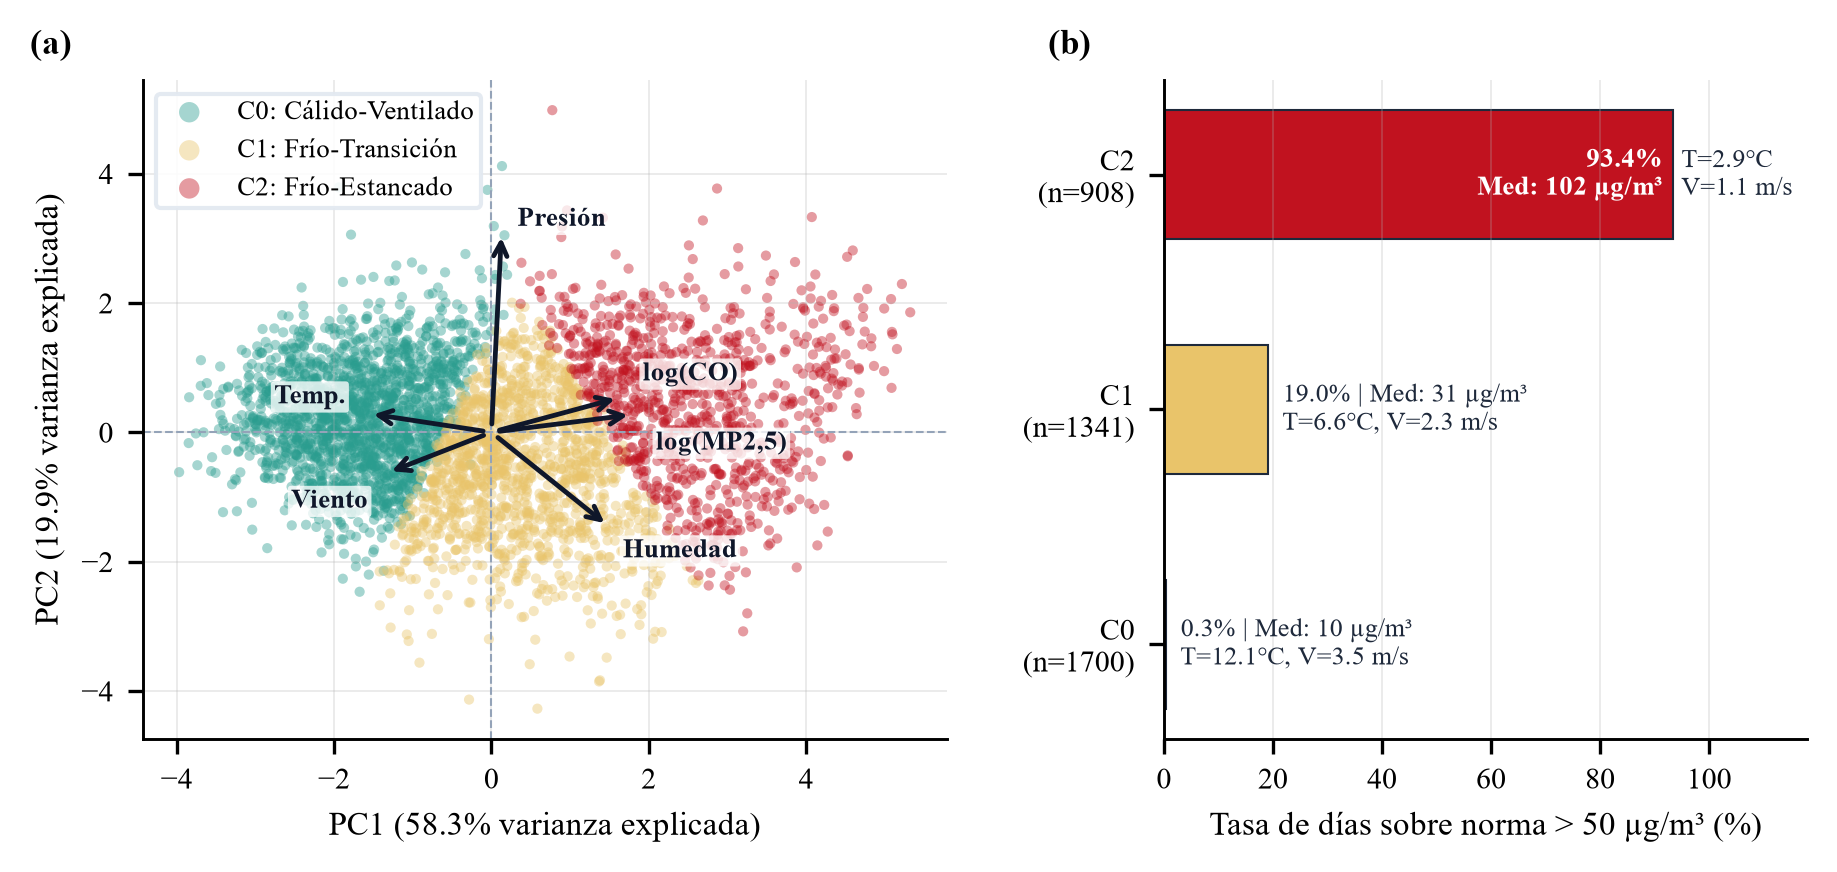
\includegraphics[width=\textwidth]{figures/fig3_pca_clusters.png}
\caption{Agrupamiento multivariado de reg{\'i}menes diarios en Coyhaique II ($n=3.949$ d{\'i}as completos, 2015--2026). (a) Biplot de las dos primeras componentes principales (78,2\% de varianza explicada) coloreado seg{\'u}n K-Means ($k=3$), con vectores de carga de las seis variables estandarizadas. (b) Tasa de excedencia ($>50$~$\mu$g/m$^3$), mediana de MP2,5, temperatura media y velocidad del viento media por r{\'e}gimen.}
\label{fig:pca}
\end{figure*}

En el an{\'a}lisis multivariado (Fig.~\ref{fig:pca}), las dos primeras componentes principales retienen el 78,2\% de la varianza (PC1: 58,3\%; PC2: 19,9\%). PC1 opone combusti{\'o}n y humedad ($\log\text{MP2,5}: +0,511$, $\log\text{CO}: +0,465$, humedad: $+0,423$) frente a temperatura ($-0,445$) y viento ($-0,380$); PC2 captura el gradiente sin{\'o}ptico de presi{\'o}n ($+0,873$) opuesto a humedad ($-0,412$). Seg{\'u}n la Tabla~\ref{tab:eval}, K-Means con $k=3$ super{\'o} a GMM y Ward en las tres m{\'e}tricas internas para $k\geq 3$ (Silueta $=0,246$, Davies--Bouldin $=1,363$, Calinski--Harabasz $=2068{,}8$) y logr{\'o} una estabilidad temporal sobresaliente ($\text{ARI}=0,974$). Aunque $k=2$ exhibe mayor silueta (0,352), solo divide el a{\~n}o en verano e invierno; $k=3$ separa tres reg{\'i}menes f{\'i}sicamente distintos (Fig.~\ref{fig:pca}b):
\begin{itemize}
\item \textit{C0 C{\'a}lido-Ventilado} ($n=1.700$; 43,0\%): mediana MP2,5 $=9{,}9$~$\mu$g/m$^3$, tasa $>50$ de 0,3\%, $T=12{,}1$~\textdegree C y viento $3{,}45$~m/s.
\item \textit{C1 Fr{\'i}o-Transici{\'o}n} ($n=1.341$; 34,0\%): mediana $30{,}7$~$\mu$g/m$^3$, tasa $>50$ de 19,0\%, $T=6{,}6$~\textdegree C, viento $2{,}31$~m/s y la menor presi{\'o}n media ($967{,}7$~hPa).
\item \textit{C2 Fr{\'i}o-Estancado} ($n=908$; 23,0\%): mediana $102{,}0$~$\mu$g/m$^3$ (media $122{,}4$), tasa $>50$ de 93,4\% ---concentrando el 76,5\% de todos los episodios--- con $T=2{,}9$~\textdegree C, viento $1{,}05$~m/s, humedad 78,3\%, CO $1{,}96$~ppm y la mayor presi{\'o}n media ($975{,}3$~hPa; 97,0\% en invierno).
\end{itemize}

\begin{table}[t]
\centering
\caption{Evaluaci{\'o}n objetiva de vistas visuales (sobre 115.200 registros) y modelos anal{\'i}ticos en Coyhaique II}
\label{tab:eval}
\scriptsize
\setlength{\tabcolsep}{3.5pt}
\begin{tabular}{@{}lcccc@{}}
\toprule
\multicolumn{5}{l}{\textbf{A. Selecci{\'o}n de m{\'e}todos visuales (puntaje 1--3 por criterio)}} \\
\midrule
M{\'e}todo visual & Perc.~\cite{cleveland1984} & Clar. & Esc. (s) & Total \\
\midrule
Serie mensual + STL & 3 & 3 & 3 (0,59 s) & \textbf{12/12}$^{\mathrm{a}}$ \\
Barras apiladas GEC & 3 & 3 & 3 (0,09 s) & \textbf{12/12}$^{\mathrm{a}}$ \\
Heatmap (hora$\times$mes) & 2 & 3 & 3 (0,08 s) & \textbf{11/12}$^{\mathrm{a}}$ \\
Calendario 13 a{\~n}os & 1 & 2 & 3 (0,04 s) & 8/12$^{\mathrm{b}}$ \\
\midrule
\multicolumn{5}{l}{\textbf{B. Agrupamiento no supervisado ($k=3$, $n=3.949$ d{\'i}as)}} \\
\midrule
Algoritmo & Silueta$\uparrow$ & DB$\downarrow$ & CH$\uparrow$ & ARI temp.$\uparrow$ \\
\midrule
\textbf{K-Means ($k=3$)} & \textbf{0,246} & \textbf{1,363} & \textbf{2068,8} & \textbf{0,974} \\
Ward ($k=3$) & 0,199 & 1,498 & 1713,6 & --- \\
GMM ($k=3$) & 0,198 & 1,557 & 1733,6 & 0,742 \\
\midrule
\multicolumn{5}{l}{\textbf{C. Validaci{\'o}n explicativa temporal (test 2024--2026, $n=1.021$)}} \\
\midrule
Modelo / atributos & F1$\uparrow$ & Prec. & Rec. & PR-AUC$\uparrow$ \\
\midrule
Persistencia ($t-1$) & 0,739 & 0,739 & 0,739 & 0,825 \\
Reg. Log. (Met.) & 0,787 & 0,652 & 0,993 & 0,936 \\
Random Forest (Met.) & 0,802 & 0,678 & 0,983 & 0,943 \\
Grad. Boost. (Met.) & 0,833 & 0,743 & 0,948 & \textbf{0,948} \\
\textbf{Grad. Boost. (Met.+lag1)} & \textbf{0,857} & \textbf{0,796} & 0,927 & 0,945 \\
\bottomrule
\multicolumn{5}{l}{\scriptsize $^{\mathrm{a}}$Incluye puntaje 3/3 en utilidad para objetivos; $^{\mathrm{b}}$utilidad 2/3 (saturaci{\'o}n en 13 a{\~n}os).}
\end{tabular}
\end{table}

La Tabla~\ref{tab:eval} sintetiza adem{\'a}s la matriz visual y la validaci{\'o}n explicativa. Todas las vistas cumplieron ampliamente el umbral de escalabilidad ($<15$~s), destacando la carga completa del esquema estrella Power BI en 0,089~s; se seleccionaron series STL, barras GEC y mapa de calor descartando el calendario multianual por menor precisi{\'o}n perceptual y saturaci{\'o}n visual. En la validaci{\'o}n fuera de muestra (2024--2026), Gradient Boosting usando {\'u}nicamente meteorolog{\'i}a y ciclo anual (\texttt{max\_depth=3}, \texttt{lr=0,08}, 100 {\'a}rboles) obtuvo $\text{F1}=0,833$ y $\text{PR-AUC}=0,948$ ($\text{ROC-AUC}=0,979$), superando ampliamente a la persistencia ($\text{F1}=0,739$). Al incorporar $\text{MP2,5}_{t-1}$ (\texttt{max\_depth=2}, \texttt{lr=0,03}, 200 {\'a}rboles), F1 ascendi{\'o} a 0,857 con precisi{\'o}n de 0,796 y sensibilidad de 0,927.

\subsection{Discusi{\'o}n}
Los resultados responden de forma coherente a los tres objetivos planteados y dialogan directamente con la literatura del sur de Chile. El ciclo horario bimodal con pico nocturno sobre 175~$\mu$g/m$^3$ en junio--julio y la fuerte co-variaci{\'o}n con CO respaldan el diagn{\'o}stico de~\cite{molina2017} y~\cite{solis2022}: la calefacci{\'o}n residencial a le{\~n}a durante tardes y noches fr{\'i}as domina la carga de MP2,5, mientras la mezcla convectiva diurna reduce las concentraciones hacia las 14:00~h.

Un hallazgo distintivo respecto a estudios previos en Coyhaique~\cite{solis2022} es la separaci{\'o}n sin{\'o}ptica entre los reg{\'i}menes invernales C1 y C2 descubierta por PCA y K-Means. En invierno las temperaturas son persistentemente bajas, por lo que el factor decisivo entre un d{\'i}a moderado (C1) y un episodio cr{\'i}tico (C2) no es solo el fr{\'i}o, sino el contraste barom{\'e}trico y e{\'o}lico: C1 agrupa jornadas con paso de sistemas frontales de baja presi{\'o}n ($967{,}7$~hPa) y viento moderado ($2{,}31$~m/s) que ventilan la cuenca, mientras C2 captura altas presiones anticicl{\'o}nicas ($975{,}3$~hPa) con calma ($1{,}05$~m/s) e inversi{\'o}n t{\'e}rmica, concordando con lo reportado para Temuco en~\cite{martinez2025}. Esto tambi{\'e}n explica que la velocidad del viento lidere la correlaci{\'o}n intra-invernal ($\rho=-0,686$) y que la sincron{\'i}a regional supere $\rho=0,82$ incluso entre Coyhaique y Cochrane, separadas por m{\'a}s de 200~km.

En el plano interanual, la ca{\'i}da sostenida entre 2014 y 2021 coincide con la entrada en vigor de medidas del Plan de Descontaminaci{\'o}n Atmosf{\'e}rica en Coyhaique; sin embargo, el estancamiento alrededor de 91--99 d{\'i}as sobre norma entre 2023 y 2026 ---y la gravedad observada en Cochrane (110--130 d{\'i}as en 2024--2025)--- advierten que el problema est{\'a} lejos de resolverse y trasciende la capital regional. Asimismo, la comparaci{\'o}n mediante ventana YTD demostr{\'o} ser indispensable: evaluar 2026 como a{\~n}o completo habr{\'i}a subestimado la media anual y ocultado el aumento de preemergencias invernales.

\subsection{Fortalezas y limitaciones}
Entre las principales fortalezas destacan el uso de 13 a{\~n}os de datos oficiales de alta completitud en la estaci{\'o}n principal, el tratamiento auditable de vac{\'i}os y del cierre parcial 2026, la integraci{\'o}n de m{\'e}todos de series de tiempo y agrupamiento validados objetivamente, y la entrega de un modelo estrella optimizado para Power BI junto a un prototipo interactivo en Python.

Entre las limitaciones se identifican: (1) ausencia de direcci{\'o}n horaria del viento en los registros SINCA, lo que impide construir rosas de viento condicionadas por episodio; (2) ausencia de series horarias de precipitaci{\'o}n y altura de capa l{\'i}mite; (3) cobertura espacial limitada a cuatro estaciones y meteorolog{\'i}a incompleta en Vialidad (60,6\%) e inexistente en Cochrane; (4) presencia de registros preliminares o no validados en 2026 (16,6\% en Coyhaique II; 31,9\% en Cochrane) y en Cochrane 2021--2023; y (5) car{\'a}cter observacional del estudio, cuyas relaciones reflejan asociaci{\'o}n estad{\'i}stica y no causalidad directa.

\section{Conclusiones}

Se caracteriz{\'o} la evoluci{\'o}n espaciotemporal de los episodios de MP2,5 y sus condiciones meteorol{\'o}gicas asociadas en la Regi{\'o}n de Ays{\'e}n (2013--2026) mediante una metodolog{\'i}a que integra auditor{\'i}a de datos faltantes, descomposici{\'o}n STL robusta, pruebas de tendencia, correlaci{\'o}n cruzada, PCA, agrupamiento K-Means y visualizaci{\'o}n interactiva orientada a Power BI.

Los resultados confirman que la contaminaci{\'o}n mantiene una fuerte estacionalidad invernal (fuerza STL $>0,80$) y un ciclo nocturno dominado por la combusti{\'o}n de le{\~n}a, en l{\'i}nea con~\cite{molina2017} y~\cite{solis2022}. Aunque Coyhaique II redujo significativamente sus d{\'i}as sobre norma entre 2014 y 2025 ($-4,93$ d{\'i}as/a{\~n}o, $p=0,002$) y Puerto Ays{\'e}n redujo sus inviernos cr{\'i}ticos ($-4,38$ d{\'i}as/a{\~n}o), el repunte invernal de 2026 en Coyhaique (99 d{\'i}as $>50$) y los altos conteos en Cochrane (hasta 130 d{\'i}as/a{\~n}o) evidencian vulnerabilidad persistente. El agrupamiento K-Means ($k=3$, $\text{ARI}=0,974$) sintetiz{\'o} la din{\'a}mica clim{\'a}tica en tres reg{\'i}menes bien diferenciados, mostrando que el estancamiento anticicl{\'o}nico con calma e{\'o}lica concentra el 76,5\% de los episodios y que la meteorolog{\'i}a explica con alta precisi{\'o}n su ocurrencia ($\text{PR-AUC}=0,948$), coherente con~\cite{martinez2025}.

Como recomendaci{\'o}n pr{\'a}ctica, la gesti{\'o}n regional de episodios deber{\'i}a extender el monitoreo meteorol{\'o}gico completo a Cochrane y publicar direcci{\'o}n horaria del viento en SINCA. Como trabajo futuro se propone incorporar registros de precipitaci{\'o}n de la Direcci{\'o}n Meteorol{\'o}gica de Chile, desplegar el informe en Power BI Service conectado a actualizaciones peri{\'o}dicas del SINCA y evaluar modelos din{\'a}micos de series de tiempo (SARIMAX) para alertas tempranas de 24 a 48 horas.

\clearpage
\bibliographystyle{IEEEtran}
\bibliography{referencias}

\end{document}
